\section{Results}\label{sec:results}
In this section we show the results of the community analysis performed in the SON gene's community by applying the metrics presented before, in \autoref{subsec:community_evaluation}.

\subsection{Relevant diseases in SON community}\label{subsec:relevant_diseases}
In \autoref{fig:diseases_son_community} we show the top 10 most relevant diseases inside the SON community:
\begin{figure}[H]
    \centering
    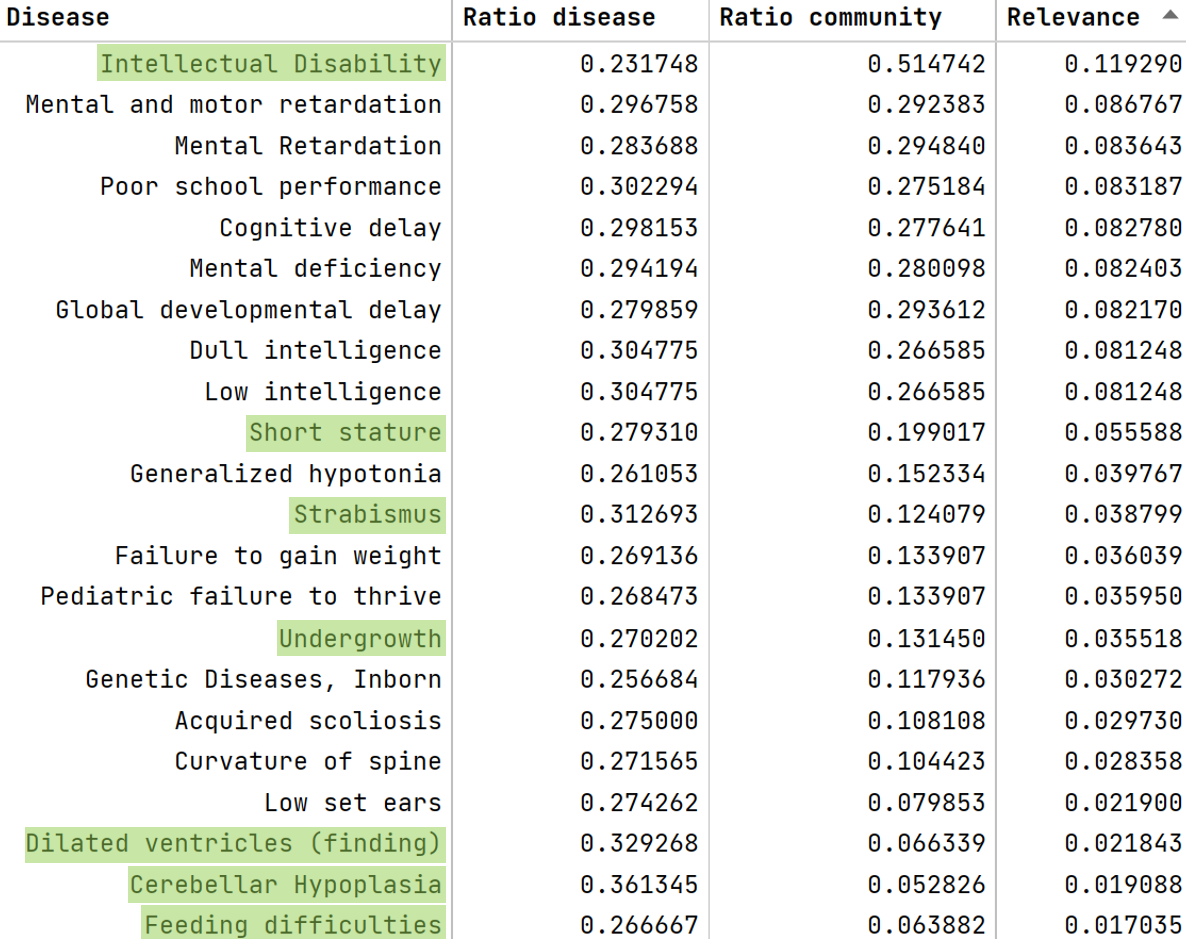
\includegraphics[width=0.9\linewidth]{images/top20_diseases_connected_highlighted.png}
    \caption{Diseases found in the SON community ordered by Relevance}
    \label{fig:diseases_son_community}
\end{figure}
Those results seems to be coherent with the state-of-the-art knowledge of the ZTTK syndrome, since most of the diseases presented in \autoref{fig:diseases_son_community} are related to neurological pathologies or cognitive difficulties, coherently with the ZTTK collateral aspects. Especially for \textit{Intellectual Disability}, encountered in $100\%$ of the ZTTK diagnoses, our results have evidenced the strong link between the two pathologies. Also, as another example, for the case of \textit{global development delay} most of the patients studied in the ZTTK paper have presented such disease.
\vspace{3mm}

With respect to all the other diseases, their relation with SON should be experimentally verified even though, apparently, they seem to align, more or less, with all the others.
\vspace{3mm}

Those results in \autoref{fig:diseases_son_community} are ordered in terms of Relevance, because of the unbalancing that could be caused by the other two metrics as discussed in \autoref{subsec:community_evaluation}: 
\begin{itemize}
    \item if we sort the rows using the "Ratio disease" we are rewarding bigger disease pathways such as \textit{Malignant breast carcinoma}, and penalizing smaller pathologies even if their overall contribution is bigger.
    \item On the other hand, sorting by "Ratio community" would only emphasize how much the disease contributes to a community without considering its pathway size, thus favoring those small disease contained entirely in a community.
\end{itemize}
 
\subsection{Diseases with SON in their pathways}\label{subsec:diseases_son}
As seen in \autoref{subsec:relevant_diseases}, most of the relevant pathologies inside SON community are well-known effects of the syndrome under inspection, now we need to focus on the disease pathways in which SON belongs to and plot them in order to confirm what we have seen until now.
\vspace{3mm}

Let's visualize directly on \autoref{fig:intellectual_disability_SON}, \autoref{fig:undergrowth_SON} and \autoref{fig:strabismus_SON} the results of our analysis, evidencing the three disease pathways inside SON gene's community. Just to point out a needed observation, the diamond nodes represents genes that belong to such pathway and we colored in orange the edges that connect them, meanwhile the SON gene was highlighted in blue to better distinguish it from the other proteins.
\begin{figure}[H]
    \centering
    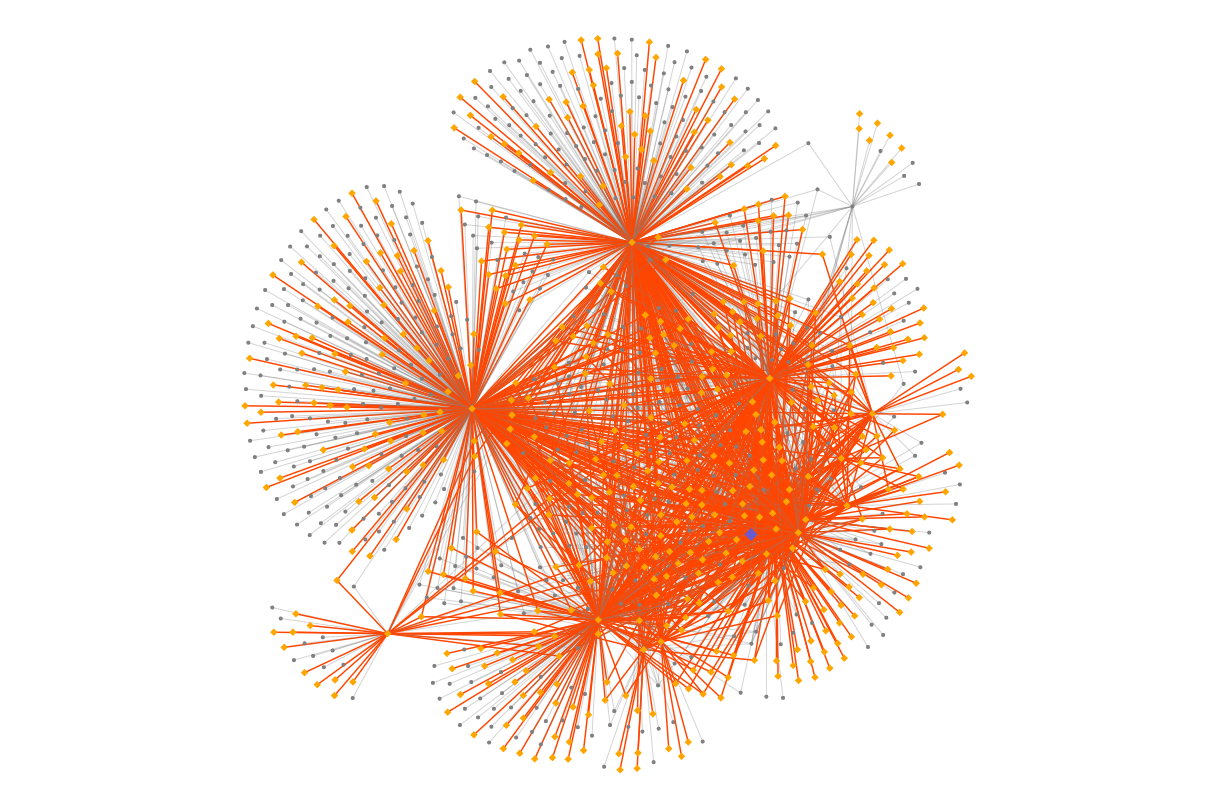
\includegraphics[width=1\linewidth]{images/plots/intellectual_disability_SON.png}
    \caption{Intellectual disability disease pathway within the SON community.}
    \label{fig:intellectual_disability_SON}
\end{figure}
Inside the community there are, more or less, $700$ nodes and it can also be noticed that the pathways are well integrated inside the community, as seen for \textit{Intellectual disability} in \autoref{fig:intellectual_disability_SON}, since its genes are connected to many hub nodes, but this was expected as that disease has the highest "Relevance" value.
\vspace{3mm}

Let's now plot in \autoref{fig:undergrowth_SON} and \autoref{fig:strabismus_SON} two more disease pathways that have SON as their gene but do not have a big "Relevance" value as the previous one.
\begin{figure}[H]
    \centering
    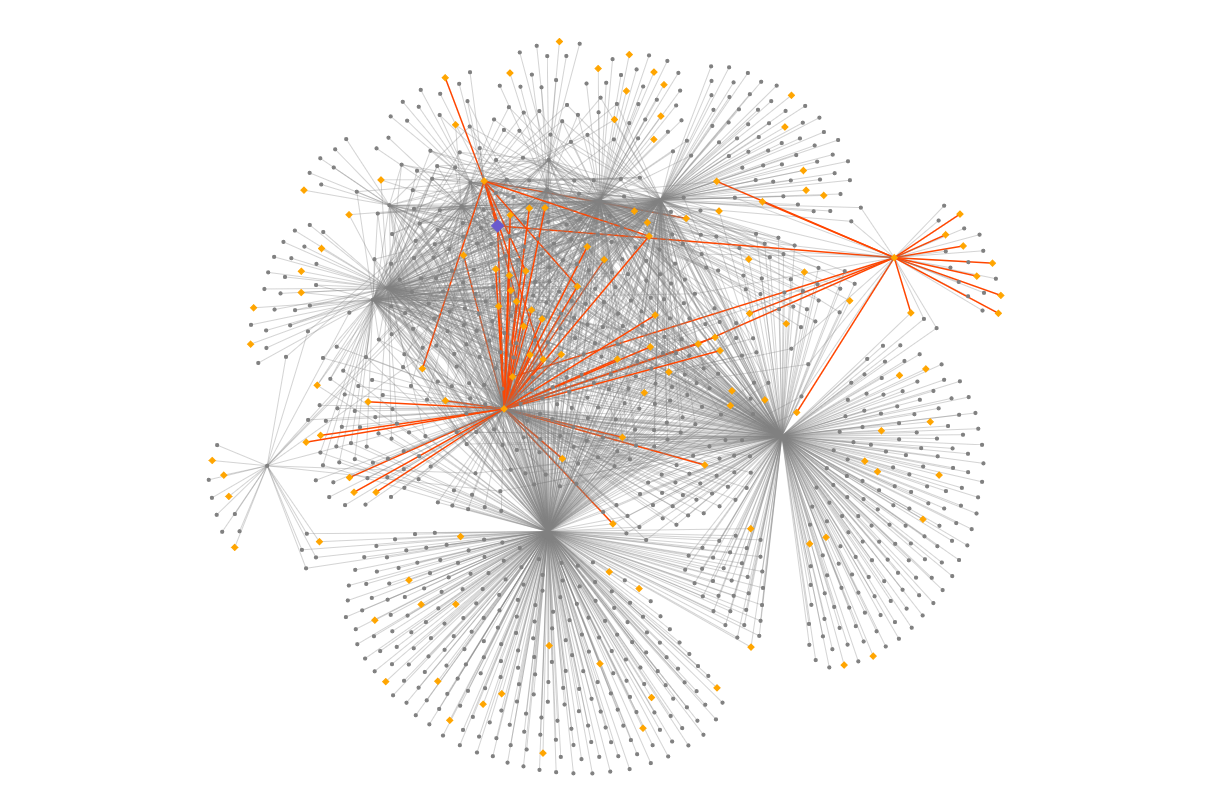
\includegraphics[width=0.8\linewidth]{images/plots/undergrowth_SON.png}
    \caption{Undergrowth disease pathway within the SON community.}
    \label{fig:undergrowth_SON}
\end{figure}

\begin{figure}[H]
    \centering
    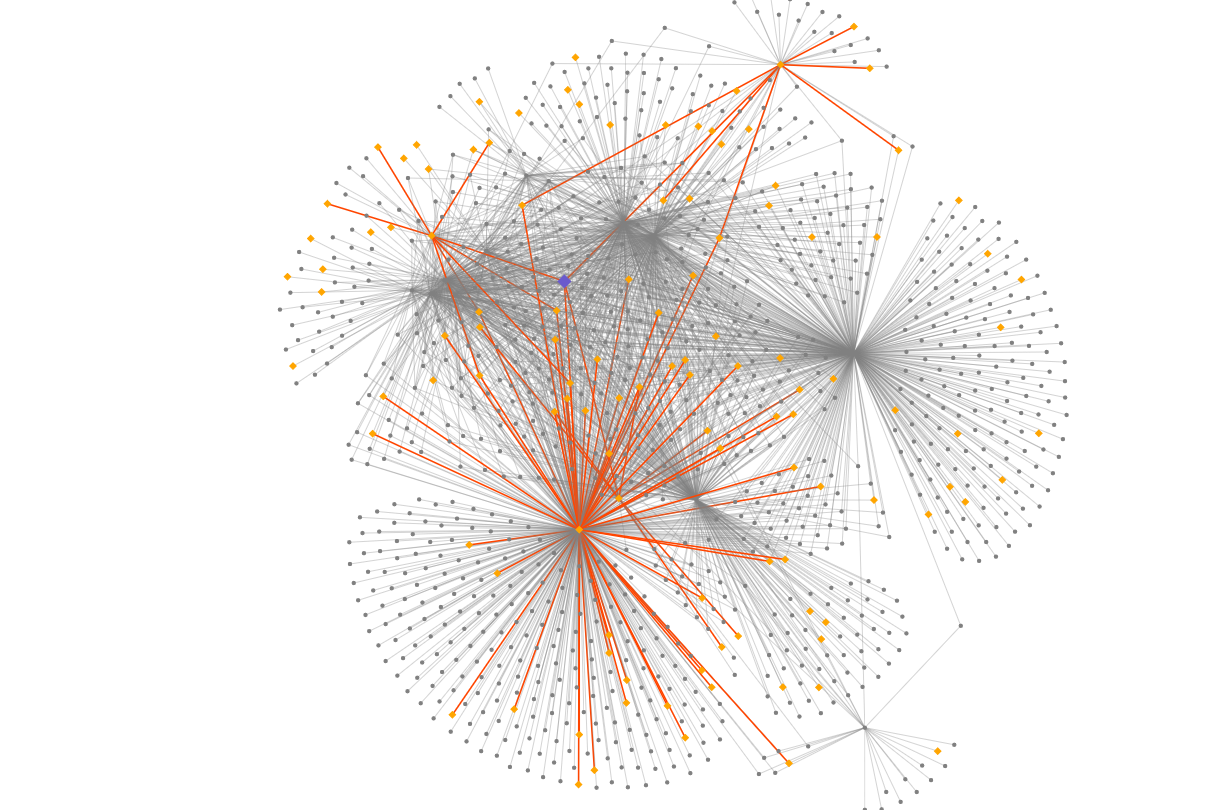
\includegraphics[width=0.8\linewidth]{images/plots/strabismus_SON.png}
    \caption{Strabismus disease pathway within the SON community.}
    \label{fig:strabismus_SON}
\end{figure}

\subsection{Diseases without SON in their pathways}\label{subsec:diseases_no_son}
To investigate potential undiscovered correlations between genes in the community and the SON gene, we will now try to explore the diseases which do not contain the latter but manifest a strong interaction in its community. In particular, it is very useful plotting these disease pathways in order to see which of them interact with SON. In \autoref{fig:top_20_diseases_disconnected} we show the collected top 20 diseases that don't have the SON gene in their pathway, ordered by the "Relevance" metric.
\begin{figure}[H]
    \centering
    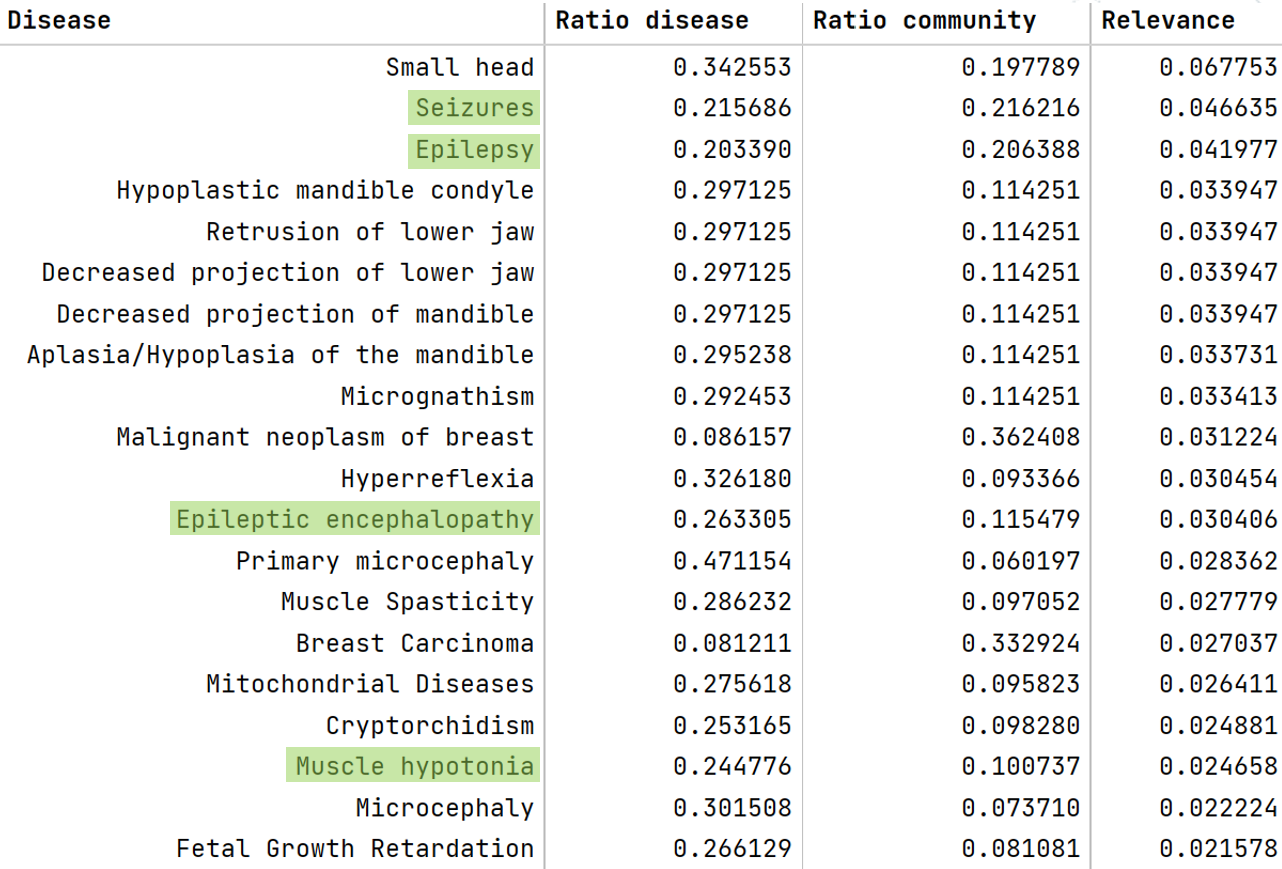
\includegraphics[width=0.8\linewidth]{images/top20_diseases_disconnected_highlighted.png}
    \caption{The top 20 diseases disconnected from SON, but in its same community.}
    \label{fig:top_20_diseases_disconnected}
\end{figure}
Beware, many of the disease we have found, do not have a known relation with ZTTK, hence their link should be experimentally verified. For the \textit{Epilepsy} disease this could be a significant result, since it has been encountered in some of the patients with ZTTK, and those results are a good signal indicating a potential relation. Even if the SON gene is not present in that pathway, at this point, it is reasonable to say that there could be a correlation and hence ZTTK patients could benefit of some of the knowledge the medical community has on epilepsy.
\vspace{3mm}

Some of the rows in \autoref{fig:top_20_diseases_disconnected} present widely studied pathologies such as various types of cancers, but their presence, as already mentioned many times (\autoref{subsec:community_evaluation}), can also derive from the influence that such big pathways have inside strict communities, even though the "Relevance" metric has a mitigation effect on it. Moreover, from the literature, we recall that there is not any proof of correlation between the ZTTK and cancer.
\vspace{3mm}

Furthermore we present some plots (\autoref{fig:small_head_NO_SON}, \autoref{fig:epilepsy_NO_SON} and \autoref{fig:hyperreflexia_NO_SON}) to evidence our results with diseases that do not have SON in their pathways but that could correlated.
\begin{figure}[H]
    \centering
    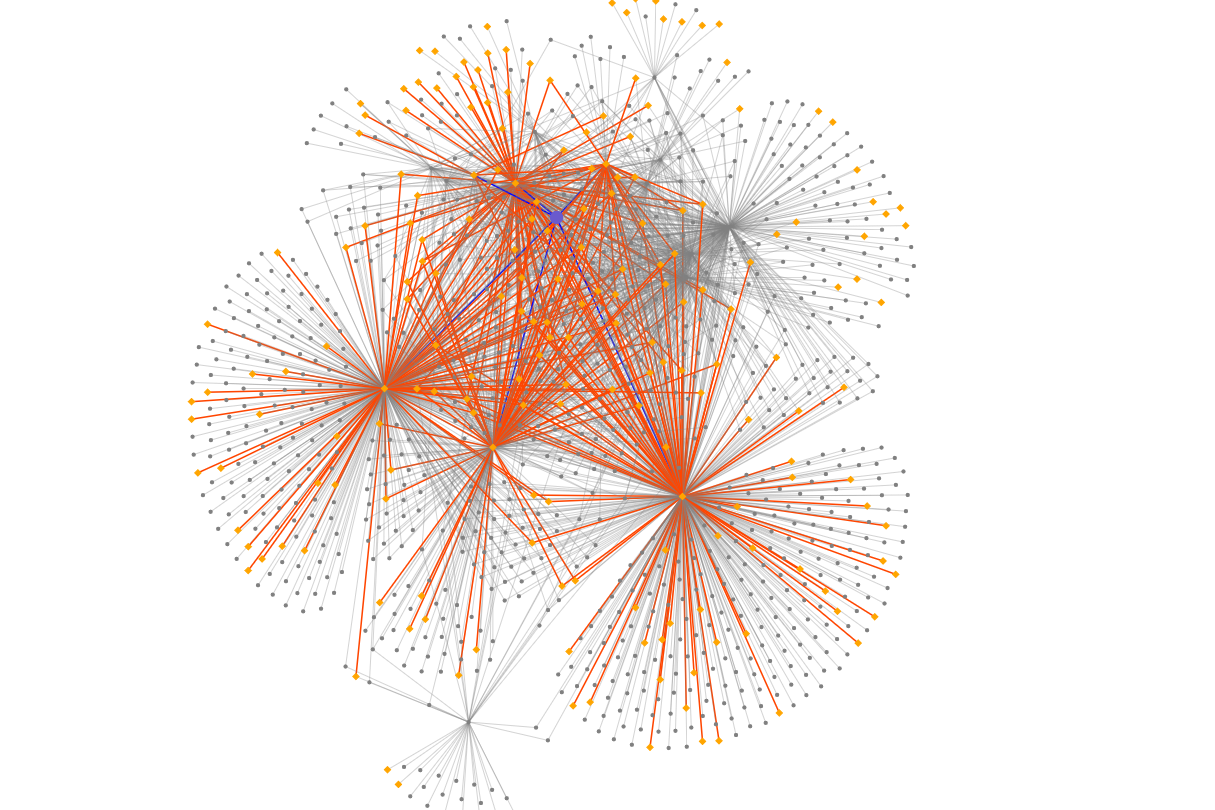
\includegraphics[width=0.8\linewidth]{images/plots/small_head_NO_SON.png}
    \caption{Small head disease pathway within the SON community. Blue edges highlights the interaction between the SON gene and the genes inside the pathway.}
    \label{fig:small_head_NO_SON}
\end{figure}

\begin{figure}[H]
    \centering
    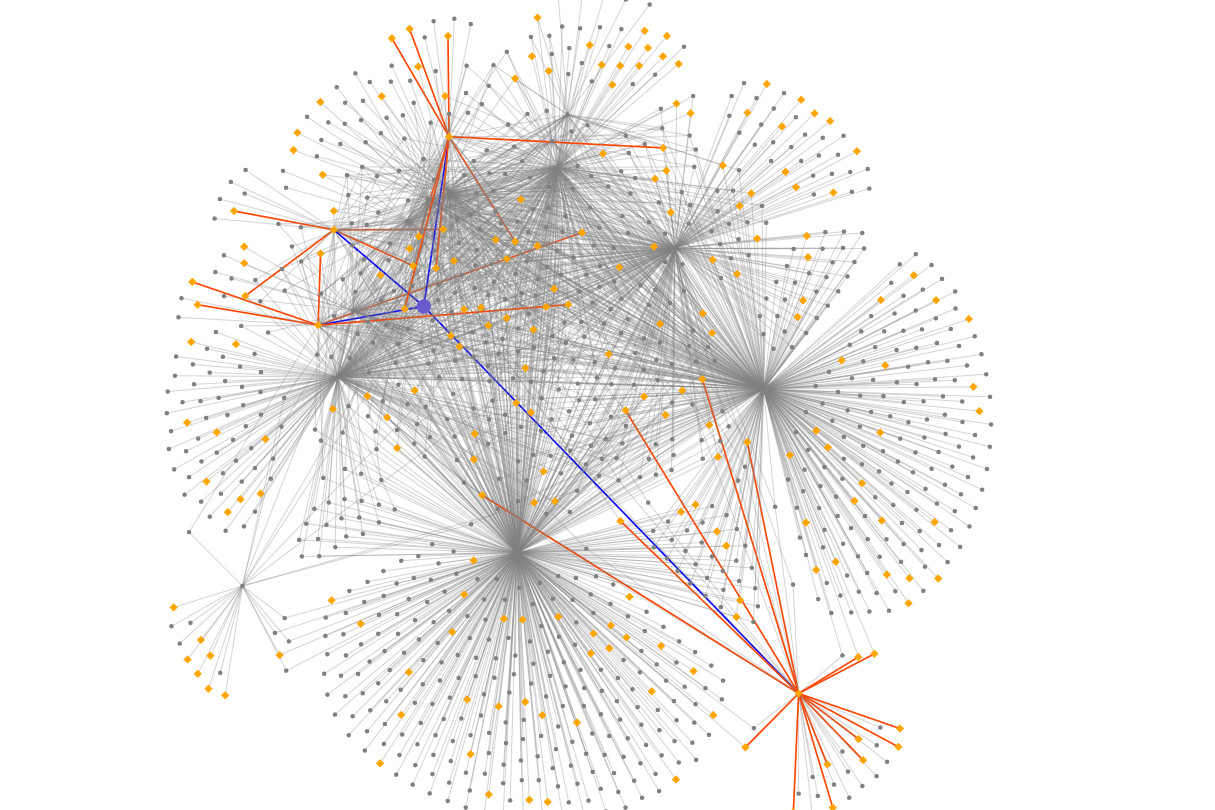
\includegraphics[width=0.8\linewidth]{images/plots/epilepsy_NO_SON.png}
    \caption{Epilepsy disease pathway within the SON community. Blue edges highlights the interaction between the SON gene and the genes inside the pathway.}
    \label{fig:epilepsy_NO_SON}
\end{figure}

\begin{figure}[H]
    \centering
    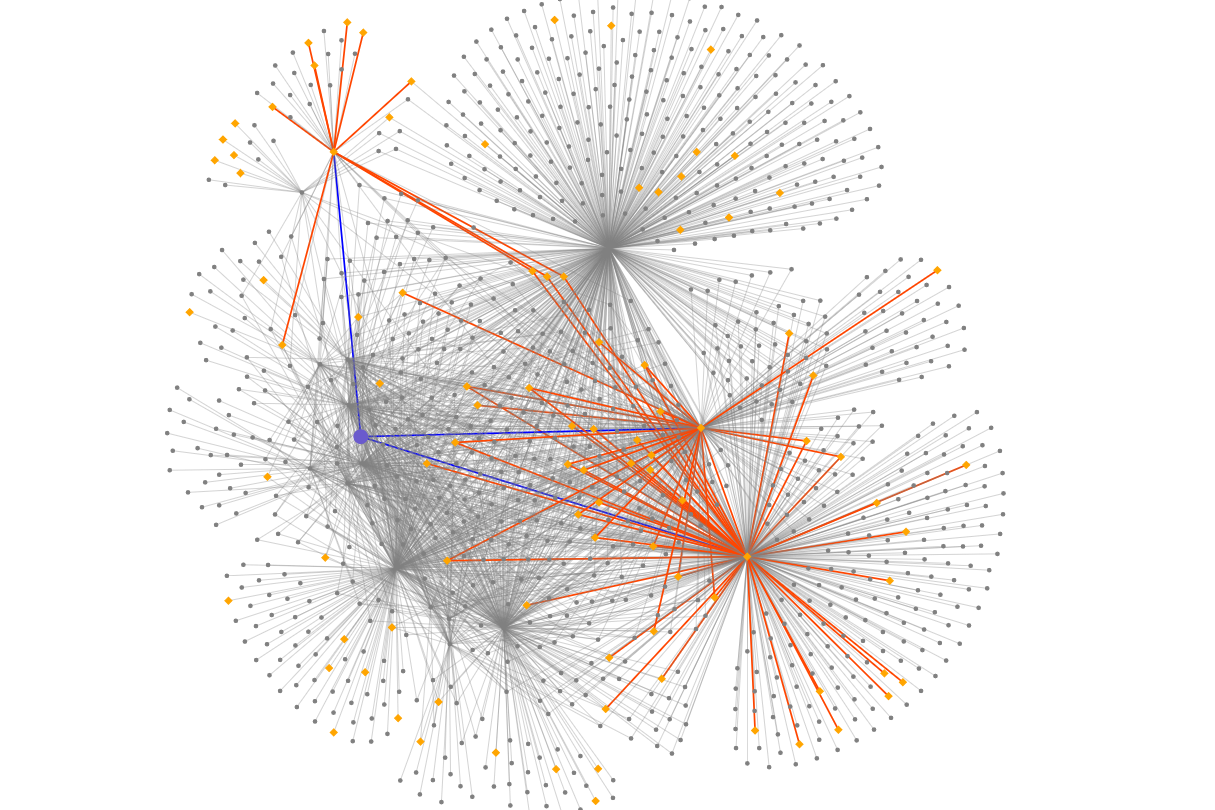
\includegraphics[width=0.8\linewidth]{images/plots/hyperreflexia_NO_SON.png}
    \caption{Hyperreflexia disease pathway within the SON community. Blue edges highlights the interaction between the SON gene and the genes inside the pathway.}
    \label{fig:hyperreflexia_NO_SON}
\end{figure}

\autoref{fig:small_head_NO_SON}, \autoref{fig:epilepsy_NO_SON} and \autoref{fig:hyperreflexia_NO_SON} could be particularly useful for experts because they point out the candidates genes to investigate on (the ones that interact with SON), we present them in \autoref{tab:disease_genes_interactions} for two chosen disease pathways.
\begin{table}[H]
\centering
\begin{tabular}{cc||cc}\hline \hline
    \multicolumn{4}{c}{\textbf{SON interactions with genes in disease pathways}} \\
    \hline \hline
    \multicolumn{2}{c||}{\textbf{Small head disease}} & \multicolumn{2}{c}{\textbf{Epilepsy}} \\
    \hline
    \textbf{Identifier} & \textbf{Name} & \textbf{Identifier} & \textbf{Name} \\
    \hline \hline
    \multirow{2}{*}{CIT} & Citron Rho-Interacting & \multirow{2}{*}{PRDM16} & Histone-Lysine  \\
    & Serine/Threonine Kinas & & N-Methyltransferase \\ \hline
    
    \multirow{2}{*}{PRDM16} & Histone-Lysine & \multirow{2}{*}{UBE2A} & Ubiquitin-Conjugating  \\
    & N-Methyltransferase & & Enzyme E2A \\ \hline
    
    \multirow{2}{*}{EFTUD2} & Elongation Factor Tu GTP & \multirow{2}{*}{NDUFAF2} & Myc-Induced \\
    & Binding Domain Containing 2 & & Mitochondrial Protein \\ \hline
    
    \multirow{2}{*}{DCPS} & Histidine Triad & \cellcolor{gray!30} & \cellcolor{gray!30} \\
    &  Nucleotide-Binding Protein 5 & \cellcolor{gray!30} & \cellcolor{gray!30} \\ \hline
    
    \multirow{2}{*}{FANCD2} & Fanconi Anemia & \cellcolor{gray!30} & \cellcolor{gray!30} \\
    & Complementation Group D2 & \cellcolor{gray!30} & \cellcolor{gray!30} \\
    \hline \hline
\end{tabular}
\caption{Genes of two diseases, \textit{Small head} and \textit{Epilepsy}, that interact with the SON gene}
\label{tab:disease_genes_interactions}
\end{table}

\subsection{Final considerations}\label{subsec:final_considerations}
For most of us this has been the first approach to bioinformatics, as such we faced many difficulties, especially in the absence of a uniform notation for the data, in the different ways each database uses to represent the knowledge. 
\vspace{3mm}

Difficulties can also be challenging, after the first, quite annoying, phase of data preparation, the following steps towards the pathway analysis were way more interesting, particularly getting in touch with real world problems and their incredible complexity. Working at something that could (in potential) be lifechanging for someone has a total different feedback and has given us much more motivation than many other works.
\vspace{3mm}

Putting aside all the difficulties, we were able to achieve what was requested and possibly discovering other diseases that might be correlated to the SON gene as shown in \autoref{subsec:diseases_no_son}, so we can say that our month-long work was useful.
